\documentclass[aspectratio=43]{beamer}

% Theme and color scheme
\usetheme{Madrid}
\usecolortheme{default}

% Packages
\usepackage[utf8]{inputenc}
\usepackage[T1]{fontenc}
\usepackage{graphicx}
\usepackage{amsmath}
\usepackage{amsfonts}
\usepackage{amssymb}
\usepackage{hyperref}
\usepackage{multicol}
\usepackage{tikz}
\usepackage{xcolor}
\usepackage{colortbl}

% Configure Beamer footnotes for citations
\setbeamerfont{footnote}{size=\scriptsize}
\setbeamertemplate{footnote}{%
  \parindent 1em\noindent%
  \raggedright
  \hbox to 1.8em{\hfil\insertfootnotemark}\insertfootnotetext\par%
}

% Citation counter for each slide
\newcounter{slidecite}
\makeatletter
\newcommand{\resetcitecounter}{\setcounter{slidecite}{0}}
% Reset counter at the beginning of each frame
\BeforeBeginEnvironment{frame}{\resetcitecounter}

% Force footnote numbering to use only Arabic numerals (no letters)
\renewcommand{\thefootnote}{\arabic{footnote}}
\makeatother

% Define citation texts as commands for reuse
\newcommand{\citeDavid}{David et al. Plant detection and counting from high-resolution RGB images acquired from UAVs. \textit{bioRxiv}, 2021}
\newcommand{\citeLiu}{Liu et al. IntegrateNet: A deep learning network for maize stand counting from UAV imagery. \textit{IEEE Geosci. Remote Sens. Lett.}, 19:6512605, 2022}
\newcommand{\citeMaizeSeeding}{Maize\_seeding dataset. \url{https://universe.roboflow.com/objectdetection-hytat/maize\_seeding}}
\newcommand{\citeMaizeSeedling}{Maize-seedling-detection dataset. \url{https://universe.roboflow.com/fyxdds-icloud-com/maize-seedling-detection}}
\newcommand{\citeFAO}{FAO. \textit{Agricultural Production Statistics 2010--2023}. FAOSTAT, Rome, Italy, 2024}
\newcommand{\citeMeier}{Meier et al. The BBCH system to coding the phenological growth stages of plants. \textit{J. Für Kult.}, 61:41--52, 2009}
\newcommand{\citeGarcia}{García-Martínez et al. Digital count of corn plants using UAVs and cross correlation. \textit{Agronomy}, 10:469, 2020}
\newcommand{\citeLeCun}{LeCun et al. Deep learning. \textit{Nature}, 521:436--444, 2015}
\newcommand{\citeFasterRCNN}{Faster R-CNN: Towards real-time object detection with region proposal networks}
\newcommand{\citeVaswani}{Vaswani et al. Attention is all you need. \textit{NIPS}, 2017}
\newcommand{\citeCarion}{Carion et al. End-to-end object detection with transformers. \textit{arXiv:2005.12872}, 2020}
\newcommand{\citeRekavandi}{Rekavandi et al. Transformers in small object detection: A benchmark and survey. \textit{arXiv:2309.04902}, 2023}
\newcommand{\citeZong}{Zong et al. DETRs with collaborative hybrid assignments training. \textit{ICCV}, 2023}
\newcommand{\citeBadgujar}{Badgujar et al. Agricultural object detection with YOLO algorithm. \textit{Comput. Electron. Agric.}, 223:109090, 2024}
\newcommand{\citeZhao}{Zhao et al. DETRs beat YOLOs on real-time object detection. \textit{arXiv:2304.08069}, 2024}
\newcommand{\citeBansal}{Bansal et al. Zero-shot object detection. \textit{ECCV}, 2018}
\newcommand{\citeHuang}{Huang et al. Survey on self-supervised few-shot learning, 2022}
\newcommand{\citeAndvaag}{Andvaag et al. Counting canola: Toward generalizable aerial plant detection. \textit{Plant Phenomics}, 6:0268, 2024}
\newcommand{\citeBarreto}{Barreto et al. Automatic UAV-based counting of seedlings. \textit{Comput. Electron. Agric.}, 191:106493, 2021}
\newcommand{\citeJiang}{Jiang et al. Deep seedling: Deep convolutional network, 2019}
\newcommand{\citeSun}{Sun et al. Revisiting unreasonable effectiveness of data in deep learning. \textit{arXiv:1707.02968}, 2017}
\newcommand{\citeAlhazmi}{Alhazmi et al. Effects of annotation quality on model performance. \textit{ICAIIC}, 2021}
\newcommand{\citeNguyen}{Nguyen et al. An evaluation of deep learning methods for small object detection. \textit{JECE}, 2020}
\newcommand{\citeBrigato}{Brigato et al. Close look at deep learning, 2020}
\newcommand{\citeDu}{Du et al. SpineNet: Learning scale-permuted backbone. \textit{CVPR}, 2020}
\newcommand{\citeRoggiolani}{Roggiolani et al. Domain-specific pre-training, 2023}
\newcommand{\citeShorten}{Shorten et al. A survey on image data augmentation for deep learning. \textit{J. Big Data}, 6:60, 2019}
\newcommand{\citeTan}{Tan et al. EfficientDet: Scalable efficient object detection, 2020}
\newcommand{\citeZhang}{Zhang et al. Comparison of YOLO-based sorghum detection, 2025}

% Custom footnote citation command - ensures numeric-only marks
\newcommand{\fcite}[1]{%
  \stepcounter{slidecite}%
  \textsuperscript{\arabic{slidecite}}%
  \footnote{#1}%
}

% Custom colors
\definecolor{lightblue}{RGB}{173,216,230}
\definecolor{lightgray}{RGB}{211,211,211}
\definecolor{uniblue}{RGB}{0,51,102}
\definecolor{highlight}{RGB}{255,153,0}

% Environmental gradient colors (define globally)
\definecolor{envlow}{RGB}{255,245,235}     % Light orange
\definecolor{envmed}{RGB}{253,174,97}      % Medium orange
\definecolor{envhigh}{RGB}{215,48,31}      % Dark red

% Set theme colors
\setbeamercolor{structure}{fg=uniblue}
\setbeamercolor{frametitle}{bg=white,fg=black}

% Custom headline: white background + thin uniblue line at the bottom
\setbeamertemplate{frametitle}{
  \nointerlineskip
  \begin{beamercolorbox}[wd=\paperwidth,ht=2.5ex,dp=1ex,left]{frametitle}
    \hspace*{2em} % Move text right
    \vspace*{-1.5ex}\strut\insertframetitle\strut
  \end{beamercolorbox}
  \hspace*{-2em} % Move line right
  {\color{uniblue}\rule{\paperwidth}{0.7mm}}
}

% Remove navigation symbols
\setbeamertemplate{navigation symbols}{}

% Remove footline
\setbeamertemplate{footline}{}

% Custom title page
\setbeamertemplate{title page}{
    \begin{picture}(0,0)
        \put(25,-220){
\includegraphics[width=0.8\paperwidth]{Imgs/Loghi.png}}
    \end{picture}
    \vfill
    \centering
    \begin{beamercolorbox}[sep=8pt,center]{title}
        \usebeamerfont{title}\inserttitle\par%
        \ifx\insertsubtitle\@empty%
        \else%
            \vskip0.25em%
            {\usebeamerfont{subtitle}\usebeamercolor[fg]{subtitle}\insertsubtitle\par}%
        \fi%
    \end{beamercolorbox}%
    \vskip1em\par
    \begin{beamercolorbox}[sep=8pt,center]{author}
        \usebeamerfont{author}\insertauthor
    \end{beamercolorbox}
    \begin{beamercolorbox}[sep=8pt,center]{institute}
        \usebeamerfont{institute}\insertinstitute
    \end{beamercolorbox}
    \begin{beamercolorbox}[sep=8pt,center]{date}
        \usebeamerfont{date}\insertdate
    \end{beamercolorbox}\vskip0.5em
    \vfill
}

% Document information
\title{Geomatic Techniques to Support Phytosanitary Products Tests whithin the EPPO Standard Framework}
\author{Samuele Bumbaca}
\institute{University of Turin}
\date{August 28, 2025}

\begin{document}

% Title slide
\begin{frame}
    \titlepage
\end{frame}

% Slide 2: The Traditional Approach to Agricultural Trials
\begin{frame}
    \frametitle{The Traditional Approach to Agricultural Trials}
    
    \begin{columns}
        \begin{column}{0.65\textwidth}
            \begin{center}
                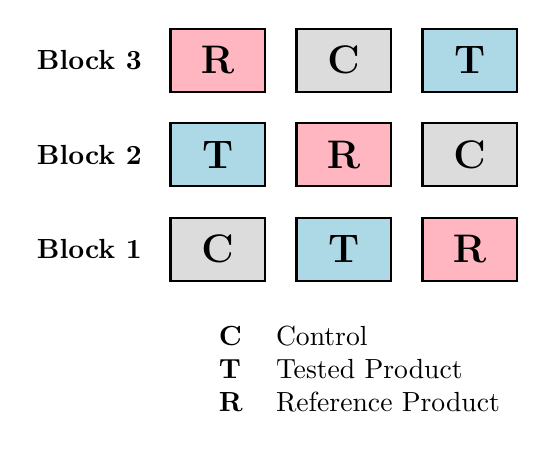
\begin{tikzpicture}[scale=0.8]
                    % Define colors for treatments
                    \definecolor{control}{RGB}{220,220,220}
                    \definecolor{tested}{RGB}{173,216,230}
                    \definecolor{reference}{RGB}{255,182,193}
                    
                    % Draw grid and plots
                    \foreach \row in {0,1,2} {
                        \foreach \col in {0,1,2} {
                            % Calculate position
                            \pgfmathsetmacro{\x}{\col*2}
                            \pgfmathsetmacro{\y}{\row*1.5}
                            
                            % Assign treatments (Latin square-like design)
                            \pgfmathsetmacro{\treatment}{int(mod(\col + \row, 3))}
                            \ifnum\treatment=0
                                \def\plotcolor{control}
                                \def\plotlabel{C}
                            \fi
                            \ifnum\treatment=1
                                \def\plotcolor{tested}
                                \def\plotlabel{T}
                            \fi
                            \ifnum\treatment=2
                                \def\plotcolor{reference}
                                \def\plotlabel{R}
                            \fi
                            
                            % Draw plot
                            \fill[\plotcolor] (\x,\y) rectangle (\x+1.5,\y+1);
                            \draw[black, thick] (\x,\y) rectangle (\x+1.5,\y+1);
                            \node at (\x+0.75,\y+0.5) {\Large\textbf{\plotlabel}};
                        }
                        % Block labels
                        \node[left] at (-0.3,\row*1.5+0.5) {\textbf{Block \pgfmathprint{int(\row+1)}}};
                    }
                    
                    % Legend
                    \node[below] at (3,-0.5) {
                        \begin{tabular}{ll}
                            \textbf{C} & Control \\
                            \textbf{T} & Tested Product \\
                            \textbf{R} & Reference Product
                        \end{tabular}
                    };
                \end{tikzpicture}
            \end{center}
        \end{column}
        
        \begin{column}{0.35\textwidth}
            \begin{block}{ANOVA Model:}
                \begin{equation*}
                    y_{ij} = \mu + \alpha_i + \beta_j + \varepsilon_{ij}
                \end{equation*}
                
                \small
                Where:
                \begin{itemize}
                    \item $y_{ij}$ = response
                    \item $\mu$ = overall mean
                    \item $\alpha_i$ = treatment effect
                    \item $\beta_j$ = block effect
                    \item $\varepsilon_{ij}$ = random error
                \end{itemize}
            \end{block}
            
            \begin{alertblock}{\tiny Note:}
                {\tiny This is the \textbf{additive model}. Modern approaches may include interaction terms: $\alpha_i \times \beta_j$}
            \end{alertblock}
        \end{column}
    \end{columns}
\end{frame}

% Slide 3: Key Assumptions of Traditional ANOVA
\begin{frame}
    \frametitle{Key Assumptions of Traditional ANOVA}
    
    \begin{block}{Statistical Assumptions:}
        \begin{itemize}
            \item \textbf{Randomization}: Treatments randomly assigned within blocks
            \item \textbf{Replication}: Each treatment appears in each block
            \item \textbf{Independence}: Observations are independent given the design
            \item \textbf{Homoscedasticity }: Equal variances across treatments
            \item \textbf{Normality}: Residuals follow normal distribution
        \end{itemize}
    \end{block}

    \begin{alertblock}{Consequences of Assumption Violations:}
        \begin{itemize}
            \item \textbf{Invalid conclusions of parametric tests}: Need for non-parametric tests leading to reduced statistical power
        \end{itemize}
    \end{alertblock}
    
    \vfill
    {\tiny
    \begin{flushleft}
        Based on R. A. Fisher, Statistical Methods for Research Workers, in S. Kotz \& N. L. Johnson (eds.), Breakthroughs in Statistics: Methodology and Distribution, pp. 66--70, Springer, New York, 1992.
    \end{flushleft}
    }
\end{frame}

% Slide 4: Right Blocking
\begin{frame}
    \frametitle{The Right Blocking: Capturing Environmental Variability}
    
    \begin{columns}
        \begin{column}{0.7\textwidth}
            \begin{center}
                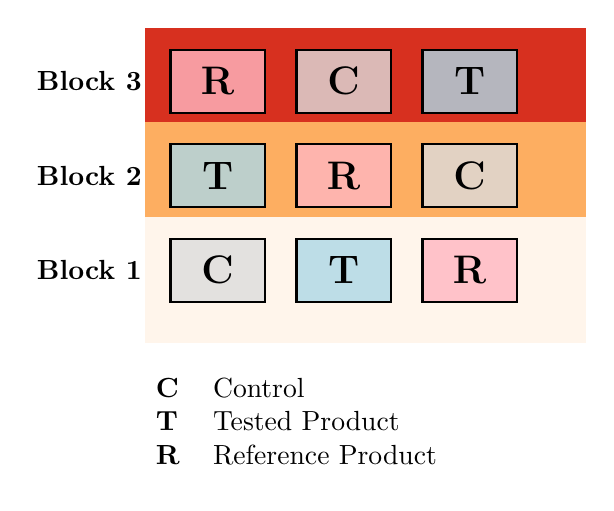
\begin{tikzpicture}[scale=0.8]
                    % Define colors for treatments
                    \definecolor{control}{RGB}{220,220,220}
                    \definecolor{tested}{RGB}{173,216,230}
                    \definecolor{reference}{RGB}{255,182,193}
                    
                    % Draw environmental variability strips (background)
                    \def\xoffset{0.1}
                    \def\yoffset{-0.15}
                    \fill[envlow] ({-0.5+\xoffset},{-0.5+\yoffset}) rectangle ({6.5+\xoffset},{1.5+\yoffset});
                    \fill[envmed] ({-0.5+\xoffset},{1.5+\yoffset}) rectangle ({6.5+\xoffset},{3+\yoffset});
                    \fill[envhigh] ({-0.5+\xoffset},{3+\yoffset}) rectangle ({6.5+\xoffset},{4.5+\yoffset});
                    
                    % Draw grid and plots
                    \foreach \row in {0,1,2} {
                        \foreach \col in {0,1,2} {
                            % Calculate position
                            \pgfmathsetmacro{\x}{\col*2}
                            \pgfmathsetmacro{\y}{\row*1.5}
                            
                            % Assign treatments (Latin square-like design)
                            \pgfmathsetmacro{\treatment}{int(mod(\col + \row, 3))}
                            \ifnum\treatment=0
                                \def\plotcolor{control}
                                \def\plotlabel{C}
                            \fi
                            \ifnum\treatment=1
                                \def\plotcolor{tested}
                                \def\plotlabel{T}
                            \fi
                            \ifnum\treatment=2
                                \def\plotcolor{reference}
                                \def\plotlabel{R}
                            \fi
                            
                            % Draw plot with some transparency to show environment
                            \fill[\plotcolor,opacity=0.8] (\x,\y) rectangle (\x+1.5,\y+1);
                            \draw[black, thick] (\x,\y) rectangle (\x+1.5,\y+1);
                            \node at (\x+0.75,\y+0.5) {\Large\textbf{\plotlabel}};
                        }
                        % Block labels
                        \node[left] at (-0.3,\row*1.5+0.5) {\textbf{Block \pgfmathprint{int(\row+1)}}};
                    }
                    
                    % Legend for treatments
                    \node[below] at (2,-1) {
                        \begin{tabular}{ll}
                            \textbf{C} & Control \\
                            \textbf{T} & Tested Product \\
                            \textbf{R} & Reference Product
                        \end{tabular}
                    };
                \end{tikzpicture}
            \end{center}
        \end{column}
        
        \begin{column}{0.3\textwidth}
            \begin{block}{\small Environmental Gradient:}
                \scriptsize
                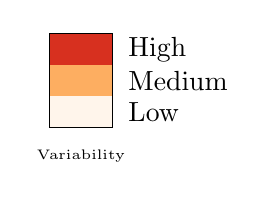
\begin{tikzpicture}[scale=0.8]
                    % Color scale bar
                    \fill[envlow] (0,0) rectangle (1,0.5);
                    \fill[envmed] (0,0.5) rectangle (1,1);
                    \fill[envhigh] (0,1) rectangle (1,1.5);
                    \draw[black] (0,0) rectangle (1,1.5);
                    
                    % Labels
                    \node[right] at (1.1,0.25) {Low};
                    \node[right] at (1.1,0.75) {Medium};
                    \node[right] at (1.1,1.25) {High};
                    \node[below] at (0.5,-0.2) {\tiny Variability};
                \end{tikzpicture}
            \end{block}
        \end{column}
    \end{columns}
    
    \begin{exampleblock}{\small Success of Blocking Strategy:}
        \begin{itemize}
            \scriptsize
            \item \textbf{Within-block homogeneity}: Treatments compared under similar conditions
            \item \textbf{Between-block heterogeneity}: Environmental gradient captured by block effects
        \end{itemize}
    \end{exampleblock}
\end{frame}

% Slide 5: The Wrong Blocking
\begin{frame}
    \frametitle{The Wrong Blocking: Assumption Violation}
    
    \begin{columns}
        \begin{column}{0.7\textwidth}
            \begin{center}
                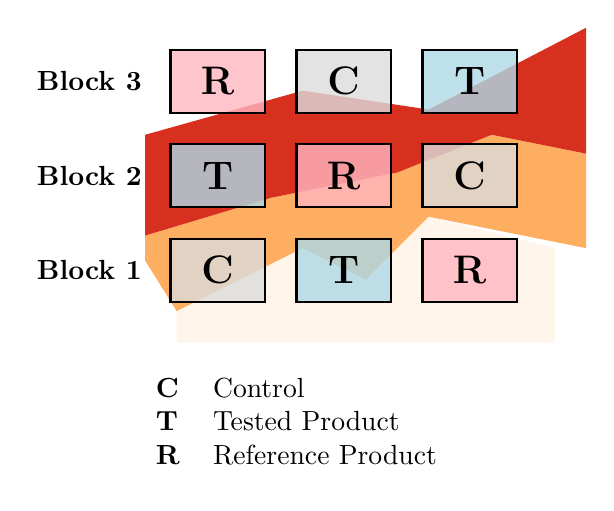
\begin{tikzpicture}[scale=0.8]
                    % Define colors for treatments
                    \definecolor{control}{RGB}{220,220,220}
                    \definecolor{tested}{RGB}{173,216,230}
                    \definecolor{reference}{RGB}{255,182,193}
                    
                    % Draw irregular environmental variability shapes (background)
                    \def\xoffset{0.1}
                    \def\yoffset{-0.15}
                    
                    % Irregular environmental patches that don't align with blocks
                    % Low variability (diagonal patches)
                    \fill[envlow] ({0+\xoffset},{0+\yoffset}) -- ({2+\xoffset},{1+\yoffset}) -- ({3+\xoffset},{0.5+\yoffset}) -- ({4+\xoffset},{1.5+\yoffset}) -- ({6+\xoffset},{1+\yoffset}) -- ({6+\xoffset},{-0.5+\yoffset}) -- ({0+\xoffset},{-0.5+\yoffset}) -- cycle;
                    
                    % Medium variability (curved patches)
                    \fill[envmed] ({-0.5+\xoffset},{1.2+\yoffset}) -- ({1.5+\xoffset},{1.8+\yoffset}) -- ({3.5+\xoffset},{2.2+\yoffset}) -- ({5+\xoffset},{2.8+\yoffset}) -- ({6.5+\xoffset},{2.5+\yoffset}) -- ({6.5+\xoffset},{1+\yoffset}) -- ({4+\xoffset},{1.5+\yoffset}) -- ({3+\xoffset},{0.5+\yoffset}) -- ({2+\xoffset},{1+\yoffset}) -- ({0+\xoffset},{0+\yoffset}) -- ({-0.5+\xoffset},{0.8+\yoffset}) -- cycle;
                    
                    % High variability (irregular top patches)
                    \fill[envhigh] ({-0.5+\xoffset},{2.8+\yoffset}) -- ({2+\xoffset},{3.5+\yoffset}) -- ({4+\xoffset},{3.2+\yoffset}) -- ({6.5+\xoffset},{4.5+\yoffset}) -- ({6.5+\xoffset},{2.5+\yoffset}) -- ({5+\xoffset},{2.8+\yoffset}) -- ({3.5+\xoffset},{2.2+\yoffset}) -- ({1.5+\xoffset},{1.8+\yoffset}) -- ({-0.5+\xoffset},{1.2+\yoffset}) -- cycle;
                    
                    % Draw grid and plots
                    \foreach \row in {0,1,2} {
                        \foreach \col in {0,1,2} {
                            % Calculate position
                            \pgfmathsetmacro{\x}{\col*2}
                            \pgfmathsetmacro{\y}{\row*1.5}
                            
                            % Assign treatments (Latin square-like design)
                            \pgfmathsetmacro{\treatment}{int(mod(\col + \row, 3))}
                            \ifnum\treatment=0
                                \def\plotcolor{control}
                                \def\plotlabel{C}
                            \fi
                            \ifnum\treatment=1
                                \def\plotcolor{tested}
                                \def\plotlabel{T}
                            \fi
                            \ifnum\treatment=2
                                \def\plotcolor{reference}
                                \def\plotlabel{R}
                            \fi
                            
                            % Draw plot with some transparency to show environment
                            \fill[\plotcolor,opacity=0.8] (\x,\y) rectangle (\x+1.5,\y+1);
                            \draw[black, thick] (\x,\y) rectangle (\x+1.5,\y+1);
                            \node at (\x+0.75,\y+0.5) {\Large\textbf{\plotlabel}};
                        }
                        % Block labels
                        \node[left] at (-0.3,\row*1.5+0.5) {\textbf{Block \pgfmathprint{int(\row+1)}}};
                    }
                    
                    % Legend for treatments
                    \node[below] at (2,-1) {
                        \begin{tabular}{ll}
                            \textbf{C} & Control \\
                            \textbf{T} & Tested Product \\
                            \textbf{R} & Reference Product
                        \end{tabular}
                    };
                \end{tikzpicture}
            \end{center}
        \end{column}
        
        \begin{column}{0.3\textwidth}
            \begin{block}{\small Environmental Gradient:}
                \scriptsize
                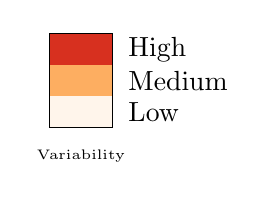
\begin{tikzpicture}[scale=0.8]
                    % Color scale bar
                    \fill[envlow] (0,0) rectangle (1,0.5);
                    \fill[envmed] (0,0.5) rectangle (1,1);
                    \fill[envhigh] (0,1) rectangle (1,1.5);
                    \draw[black] (0,0) rectangle (1,1.5);
                    
                    % Labels
                    \node[right] at (1.1,0.25) {Low};
                    \node[right] at (1.1,0.75) {Medium};
                    \node[right] at (1.1,1.25) {High};
                    \node[below] at (0.5,-0.2) {\tiny Variability};
                \end{tikzpicture}
            \end{block}
        \end{column}
    \end{columns}
    
    \begin{alertblock}{\small Heteroscedasticity Assumption Violation Problem:}
        \scriptsize
        \begin{itemize}
            \item \textbf{Blocks fail to capture environmental variability}: Treatments compared under different conditions
            \item \textbf{Invalid parametric test}: Residual variance differs across treatments
        \end{itemize}
    \end{alertblock}
\end{frame}

% Slide 6: The Problem
\begin{frame}
    \frametitle{Current Limitations in Statistics for Agricultural Trials}
    
    \begin{block}{Traditional Approach Issues:}
        \begin{itemize}
            \item \textbf{Human-dependent blocking}: Environmental variability assessment relies on experimenter experience
            \item \textbf{A priori identification}: Must identify variance sources BEFORE data collection
        \end{itemize}
    \end{block}
    
    \begin{alertblock}{The Challenge:}
        \textit{How can we capture environmental variability mathematically rather than through human judgment?}
    \end{alertblock}
\end{frame}

% Slide 7: Geostatistical Approach
\begin{frame}
    \frametitle{Geostatistical Approach: Spatial Linear Mixed Models}
    
    \begin{columns}
        \begin{column}{0.65\textwidth}
            \begin{center}
                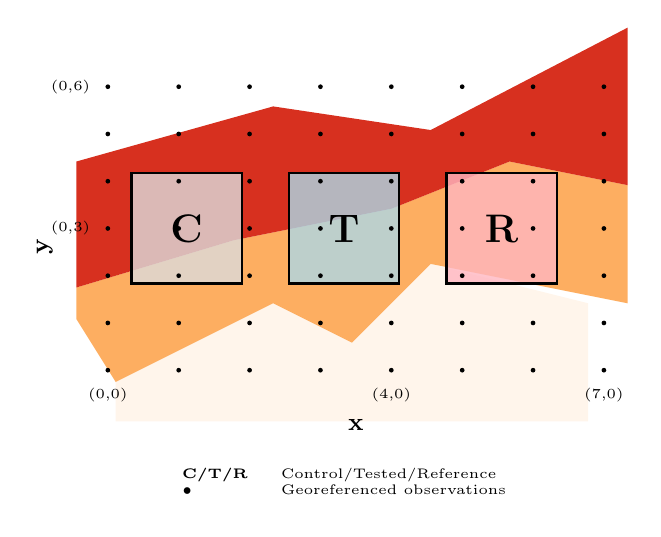
\begin{tikzpicture}[scale=1]
                    % Define colors for treatments
                    \definecolor{control}{RGB}{220,220,220}
                    \definecolor{tested}{RGB}{173,216,230}
                    \definecolor{reference}{RGB}{255,182,193}
                    
                    % Draw irregular environmental variability shapes (background)
                    \def\xoffset{0.1}
                    \def\yoffset{-0.15}
                    
                    % Same irregular environmental patches as slide 5
                    \fill[envlow] ({0+\xoffset},{0+\yoffset}) -- ({2+\xoffset},{1+\yoffset}) -- ({3+\xoffset},{0.5+\yoffset}) -- ({4+\xoffset},{1.5+\yoffset}) -- ({6+\xoffset},{1+\yoffset}) -- ({6+\xoffset},{-0.5+\yoffset}) -- ({0+\xoffset},{-0.5+\yoffset}) -- cycle;
                    
                    \fill[envmed] ({-0.5+\xoffset},{1.2+\yoffset}) -- ({1.5+\xoffset},{1.8+\yoffset}) -- ({3.5+\xoffset},{2.2+\yoffset}) -- ({5+\xoffset},{2.8+\yoffset}) -- ({6.5+\xoffset},{2.5+\yoffset}) -- ({6.5+\xoffset},{1+\yoffset}) -- ({4+\xoffset},{1.5+\yoffset}) -- ({3+\xoffset},{0.5+\yoffset}) -- ({2+\xoffset},{1+\yoffset}) -- ({0+\xoffset},{0+\yoffset}) -- ({-0.5+\xoffset},{0.8+\yoffset}) -- cycle;
                    
                    \fill[envhigh] ({-0.5+\xoffset},{2.8+\yoffset}) -- ({2+\xoffset},{3.5+\yoffset}) -- ({4+\xoffset},{3.2+\yoffset}) -- ({6.5+\xoffset},{4.5+\yoffset}) -- ({6.5+\xoffset},{2.5+\yoffset}) -- ({5+\xoffset},{2.8+\yoffset}) -- ({3.5+\xoffset},{2.2+\yoffset}) -- ({1.5+\xoffset},{1.8+\yoffset}) -- ({-0.5+\xoffset},{1.2+\yoffset}) -- cycle;
                    
                    % Add treatment rectangles in center Y of plot (larger rectangles)
                    \pgfmathsetmacro{\midY}{1.8}
                    \fill[color=control,opacity=0.8] (0.3,\midY-0.7) rectangle (1.7,\midY+0.7);
                    \draw[black, thick] (0.3,\midY-0.7) rectangle (1.7,\midY+0.7);
                    \node at (1,\midY) {\Large\textbf{C}};
                    
                    \fill[color=tested,opacity=0.8] (2.3,\midY-0.7) rectangle (3.7,\midY+0.7);
                    \draw[black, thick] (2.3,\midY-0.7) rectangle (3.7,\midY+0.7);
                    \node at (3,\midY) {\Large\textbf{T}};
                    
                    \fill[color=reference,opacity=0.8] (4.3,\midY-0.7) rectangle (5.7,\midY+0.7);
                    \draw[black, thick] (4.3,\midY-0.7) rectangle (5.7,\midY+0.7);
                    \node at (5,\midY) {\Large\textbf{R}};
                    
                    % Draw grid of observation points with coordinates (denser grid)
                    \foreach \row in {0,1,2,3,4,5,6} {
                        \foreach \col in {0,1,2,3,4,5,6,7} {
                            % Calculate position (adjusted for denser grid)
                            \pgfmathsetmacro{\x}{\col*0.9}
                            \pgfmathsetmacro{\y}{\row*0.6}
                            
                            % Draw observation point
                            \fill[black] (\x,\y) circle (0.03);
                            
                            % Add coordinate labels for some points (adjusted for new grid)
                            \ifnum\row=0
                                \ifnum\col=0
                                    \node[below, font=\tiny] at (\x,\y-0.1) {(0,0)};
                                \fi
                                \ifnum\col=4
                                    \node[below, font=\tiny] at (\x,\y-0.1) {(4,0)};
                                \fi
                                \ifnum\col=7
                                    \node[below, font=\tiny] at (\x,\y-0.1) {(7,0)};
                                \fi
                            \fi
                            \ifnum\col=0
                                \ifnum\row=3
                                    \node[left, font=\tiny] at (\x-0.1,\y) {(0,3)};
                                \fi
                                \ifnum\row=6
                                    \node[left, font=\tiny] at (\x-0.1,\y) {(0,6)};
                                \fi
                            \fi
                        }
                    }
                    
                    % Axis labels
                    \node[below, font=\small] at (3.15,-0.5) {\textbf{x}};
                    \node[left, font=\small, rotate=90] at (-0.8,1.8) {\textbf{y}};
                    
                    % Legend for treatments and spatial data
                    \node[below, font=\tiny] at (3,-1.1) {
                        \begin{tabular}{ll}
                            \textbf{C/T/R} & Control/Tested/Reference \\
                            \textbf{\(\bullet\)} & Georeferenced observations
                        \end{tabular}
                    };

                \end{tikzpicture}
            \end{center}
        \end{column}
        
        \begin{column}{0.35\textwidth}
            \begin{block}{\small Spatial LMM:}
                \begin{equation*}
                    y(s_i) = \mu + \alpha_j + f(s_i) + \varepsilon_i
                \end{equation*}
                
                \scriptsize
                Where:
                \begin{itemize}
                    \item $y(s_i)$ = response at $s_i$
                    \item $\mu$ = overall mean
                    \item $\alpha_j$ = treatment effect
                    \item $f(s_i)$ = spatial random field
                    \item $\varepsilon_i$ = error
                    \item $s_i = (x_i, y_i)$  = coordinates
                \end{itemize}
            \end{block}
            
        \end{column}
    \end{columns}
    
    \begin{exampleblock}{\scriptsize Benefits:}
        \tiny
        \begin{itemize}
            \item \textbf{No blocking}: Spatial correlation captures variability
            \item \textbf{Post-hoc}: No a priori variance identification
            \item \textbf{Homoscedasticity}: Assumption satisfied in more cases in respect blocking
        \end{itemize}
    \end{exampleblock}
\end{frame}

% Slide 8: Statistical Methods Comparison: Introduction
\begin{frame}
    \frametitle{Statistical Methods Comparison: Introduction}
    
    \begin{block}{Comparison Objective:}
        Evaluate the performance of \textbf{traditional RCBD} versus \textbf{spatial geostatistical methods} (SpATS) in capturing environmental variability and estimating treatment effects.
    \end{block}
    
    \begin{columns}
        \begin{column}{0.5\textwidth}
            \begin{exampleblock}{Synthetic Dataset:}
                \begin{itemize}
                    \item \textbf{\small 54 observations}\small (6×9 grid)
                    \item \textbf{\small 3 treatments}\small : Control (0 t/ha), Reference (0.5 t/ha), Test (1.0 t/ha)
                    \item \textbf{\small 3 blocks}\small (18 plots each)
                    \item \textbf{\small Environmental zones}\small : Low (-1.5 t/ha), Medium (0 t/ha), High (+1.5 t/ha)
                \end{itemize}
            \end{exampleblock}
        \end{column}
        
        \begin{column}{0.5\textwidth}
            \begin{alertblock}{Tested Models:}
                \begin{enumerate}
                    \item \textbf{RCBD Model}: Linear Mixed Model with random block effects
                    \begin{equation*}
                        y_{ij} = \mu + \alpha_i + \beta_j + \varepsilon_{ij}
                    \end{equation*}
                    
                    \item \textbf{SpATS Model}: Spatial model with PSANOVA splines
                    \begin{equation*}
                        y(s) = \mu + \alpha_i + f(s) + \varepsilon(s)
                    \end{equation*}
                \end{enumerate}
            \end{alertblock}
        \end{column}
    \end{columns}
    
    \vspace{0.3cm}
    \begin{center}
        \small Where: $\alpha_i$ = treatment effects, $\beta_j$ = block effects, $f(s)$ = spatial smooth function, $s$ = coordinates
    \end{center}
\end{frame}

% Slide 9: Statistical Methods Comparison: The Field Trial
\begin{frame}
    \frametitle{Statistical Methods Comparison: The Field Trial Design}
    
    \begin{center}
        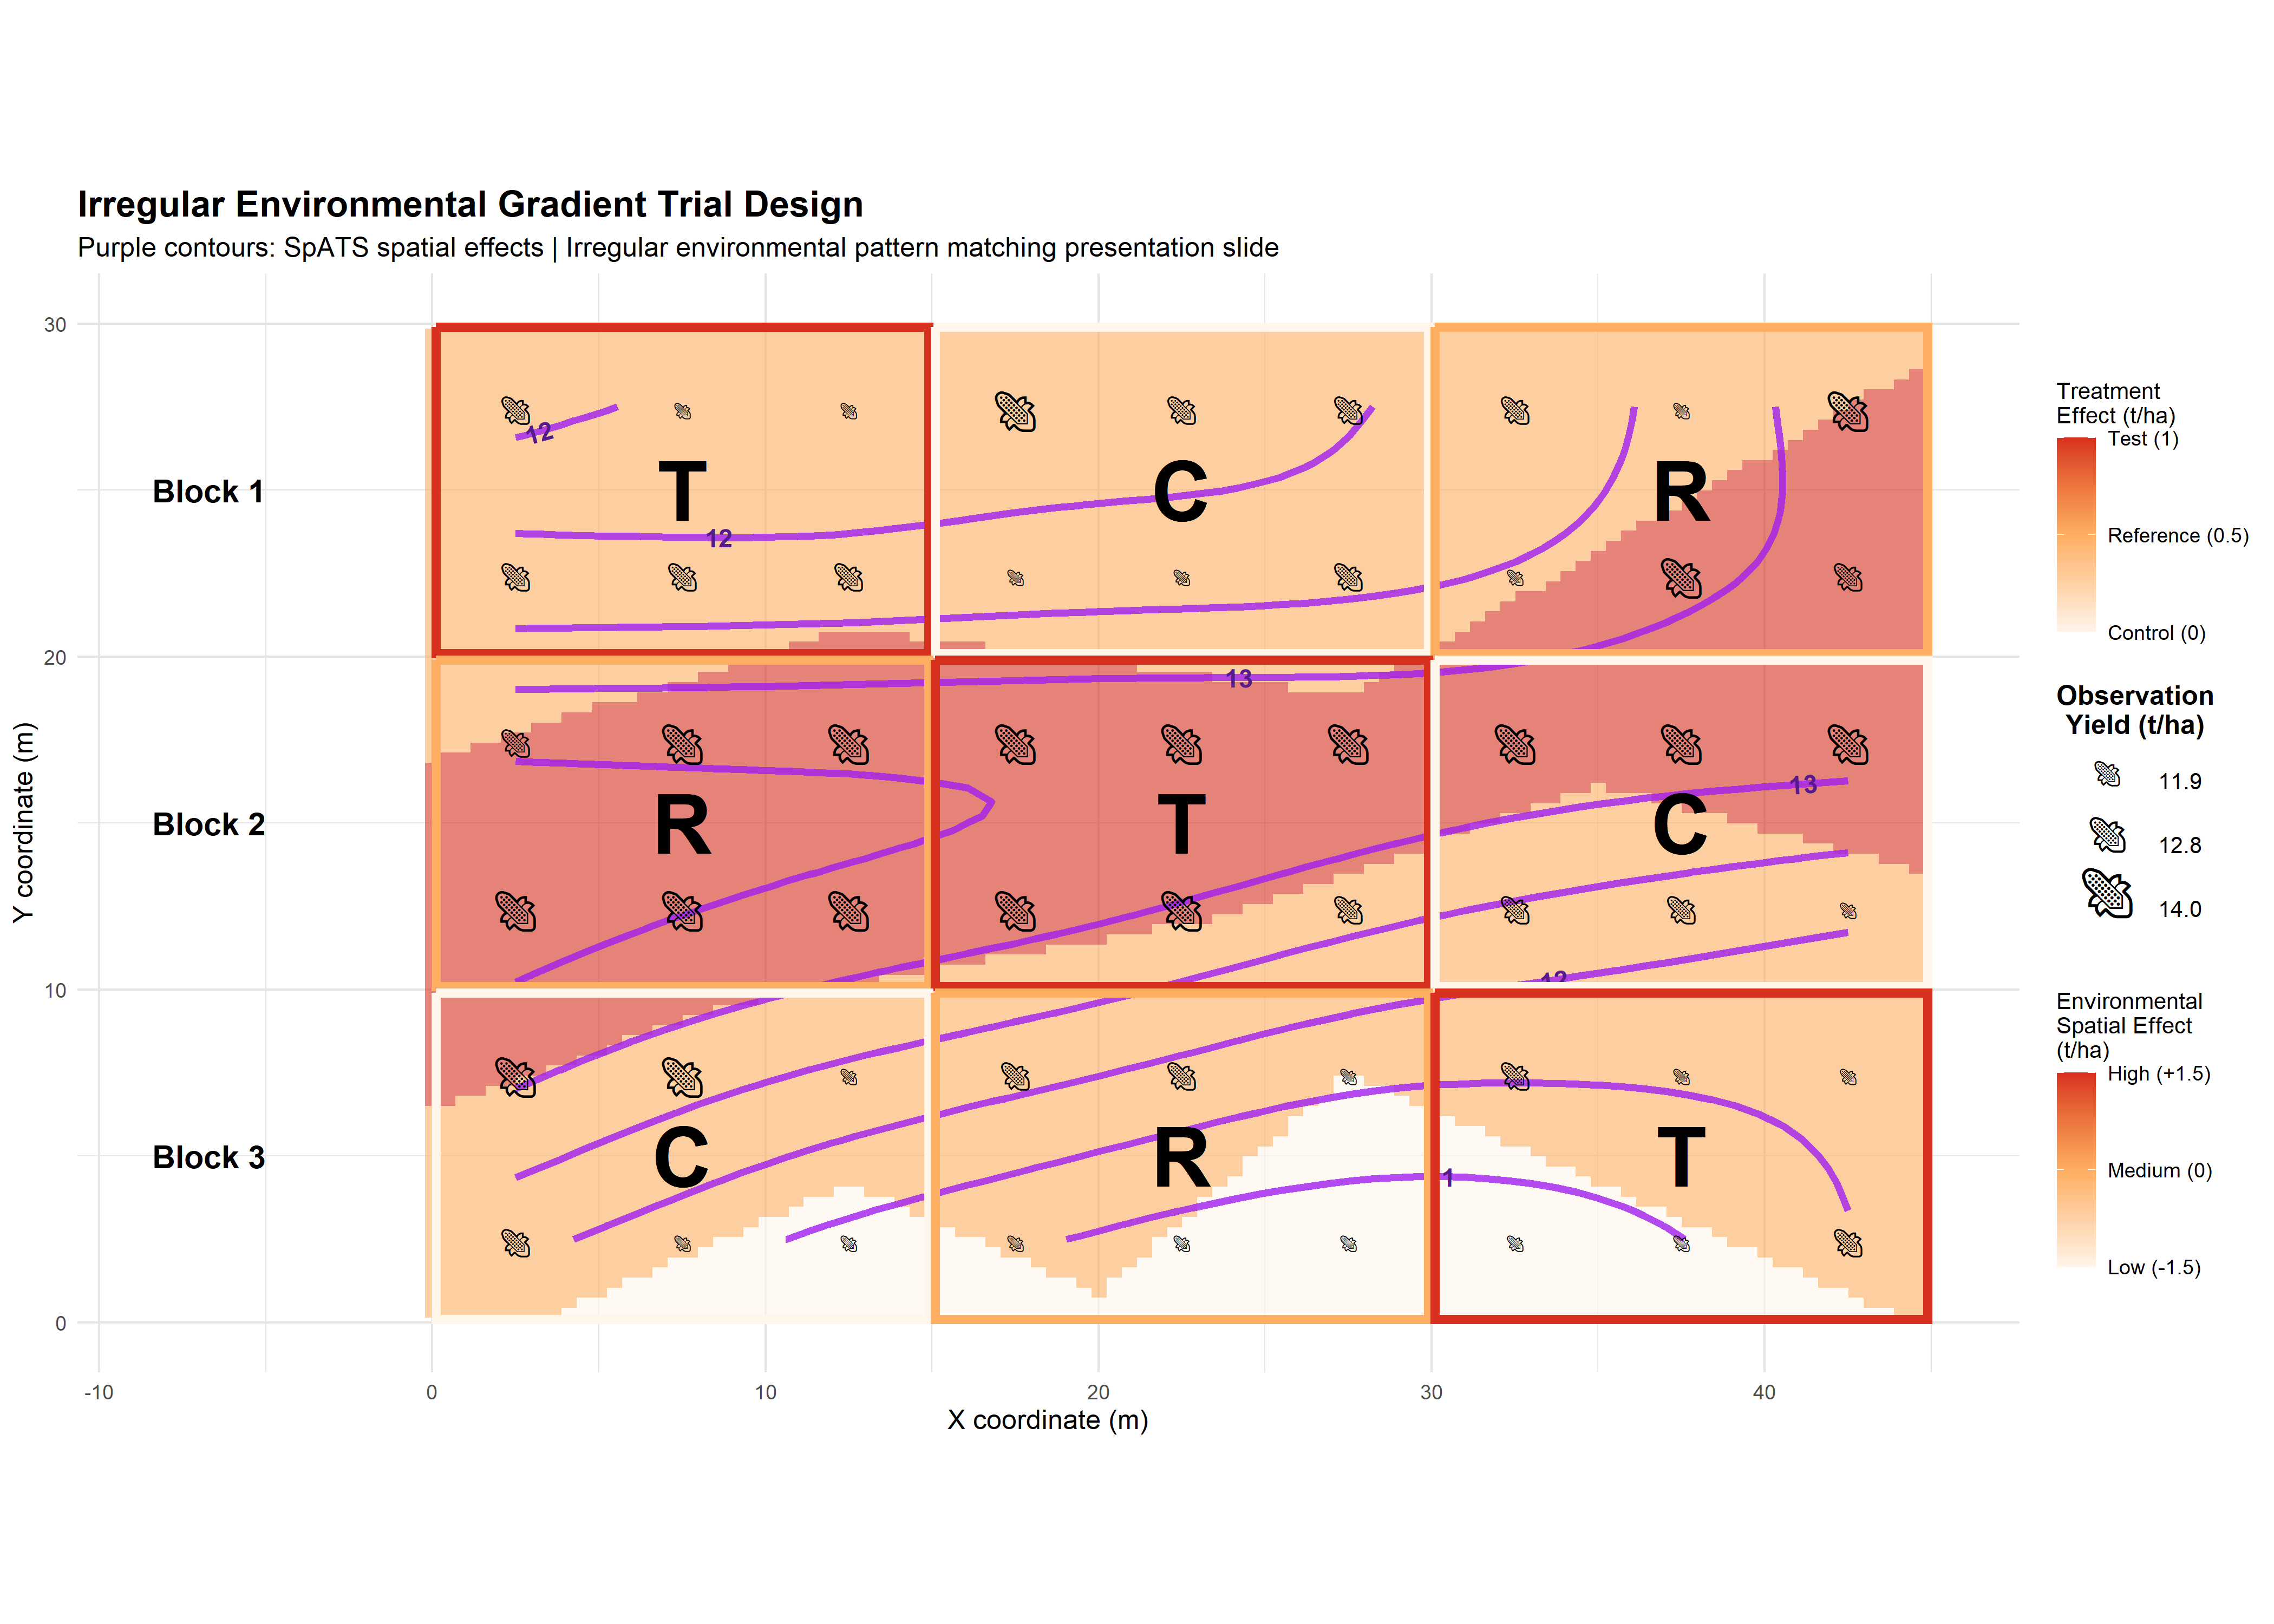
\includegraphics[width=0.95\textwidth]{Imgs/integrated_rcbd_spats_comparison_irregular.png}
    \end{center}
    
    \begin{block}{\small Legend Interpretation:}
        \begin{columns}
            \begin{column}{0.33\textwidth}
                \textbf{Background Raster:}
                \begin{itemize}
                    \scriptsize
                    \item Environmental spatial effects
                    \item Irregular zones: Low/Medium/High
                    \item White to orange to red gradient
                \end{itemize}
            \end{column}
            
            \begin{column}{0.33\textwidth}
                \textbf{Purple Contours:}
                \begin{itemize}
                    \scriptsize
                    \item SpATS estimated spatial effects
                    \item Smooth spline interpolation
                    \item Continuous spatial modeling
                \end{itemize}
            \end{column}
            
            \begin{column}{0.33\textwidth}
                \textbf{Plot Elements:}
                \begin{itemize}
                    \scriptsize
                    \item \textbf{Rectangles}: Treatment effect magnitude (colored borders)
                    \item \textbf{Letters}: C/T/R treatments
                    \item \textbf{Corn symbols}: Individual yield observations (sized by value)
                \end{itemize}
            \end{column}
        \end{columns}
    \end{block}
\end{frame}

% Slide 10: Statistical Methods Comparison: Results
\begin{frame}
    \frametitle{Statistical Methods Comparison: Results}
    
    \begin{columns}
        \begin{column}{0.5\textwidth}
            \begin{block}{\small Model Performance \scriptsize (Mean Absolute Errors tonn/ha):}
                \begin{table}[h]
                    \centering
                    \scriptsize
                    \begin{tabular}{lcc}
                        \hline
                        \textbf{Model} & \textbf{Treat. Error} & \textbf{Env. Error} \\
                        \hline
                        RCBD Model & 0.13 & 0.62 \\
                        SpATS Spatial & 0.03 & 0.45 \\
                        \hline
                    \end{tabular}
                \end{table}
            \end{block}
            
            \begin{exampleblock}{\small Treatment Effect Estimation (tonn/ha):}
                \begin{table}[h]
                    \centering
                    \scriptsize
                    \begin{tabular}{lccc}
                        \hline
                        \textbf{Treatment} & \textbf{True} & \textbf{RCBD} & \textbf{SpATS} \\
                        \hline
                        Control & 0.00 & 0.00 & 0.00 \\
                        Reference & 0.50 & 0.40 & 0.45 \\
                        Test & 1.0 & 0.69 & 0.94 \\
                        \hline
                    \end{tabular}
                \end{table}
            \end{exampleblock}
        \end{column}
        
        \begin{column}{0.5\textwidth}
            \begin{alertblock}{\small Key Findings:}
                \begin{itemize}
                    \footnotesize
                    \item \textbf{Both models satisfied assumptions}
                    \item \textbf{SpATS outperformed RCBD}:
                    \begin{itemize}
                        \scriptsize
                        \item 3.8× better treatment effect estimation
                        \item 1.4× better environmental effect estimation
                    \end{itemize}
                    \item \textbf{RCBD underestimated} by 20-31\%
                    \item \textbf{SpATS <6\% error}
                \end{itemize}
            \end{alertblock}
            
            \begin{block}{\small Implications:}
                \scriptsize
                Even when traditional RCBD meets statistical assumptions, \textbf{spatial modeling provides superior accuracy} in treatment effect estimation by properly accounting for environmental spatial variability.
            \end{block}
        \end{column}
    \end{columns}
\end{frame}

% Slide 11: Research Gap
\begin{frame}
    \frametitle{The Missing Link: Spatial Coordinates}
    
    \begin{columns}
        \begin{column}{0.5\textwidth}
            \begin{block}{Geostatistical Methods Advantages:}
                \begin{itemize}
                    \item[\textcolor{green}{\checkmark}] \textbf{Mathematical modeling} of environmental variability
                    \item[\textcolor{green}{\checkmark}] \textbf{Post-hoc analysis} - no need for prior knowledge of the environment variables and of their distribution
                    \item[\textcolor{green}{\checkmark}] \textbf{Superior performance} in handling spatial heterogeneity
                    \item[\textcolor{green}{\checkmark}] \textbf{EPPO recognized} approach \scriptsize (PP1/152(4) - Design and analysis of efficacy evaluation trials)
                \end{itemize}
            \end{block}
        \end{column}
        
        \begin{column}{0.5\textwidth}
            \begin{alertblock}{Current Barrier:}
                \begin{itemize}
                    \item[\textcolor{red}{\(\times\)}] \textbf{Requires spatially referenced observations}
                    \item[\textcolor{red}{\(\times\)}] \textbf{Traditional manual assessments lack coordinates}
                    \item[\textcolor{red}{\(\times\)}] \textbf{Implementation gap} in practical field trials
                \end{itemize}
            \end{alertblock}
        \end{column}
    \end{columns}
\end{frame}

% Slide 12: Research Question
\begin{frame}
    \frametitle{Central Research Question}
    
    \begin{exampleblock}{}
        \large
        \textbf{Can geomatics technologies provide spatially referenced observations that enable geostatistical analysis within EPPO-compliant Plant Protection Product trials?}
    \end{exampleblock}
    
    \vspace{1em}
    
    \begin{block}{Specific Objectives:}
        \begin{enumerate}
            \item Establish which geomatics technologies can be used to collect spatially referenced observations
            \item Demonstrate the feasibility of collect spatially referenced observations in compliant with EPPO standards
            \item Validate performance against traditional methods
            \item Provide practical implementation guidelines
        \end{enumerate}
    \end{block}
\end{frame}

% Slide 13: Geomatic Techniques
\begin{frame}
    \frametitle{\small Geomatic Technologies: Workflow for Spatially Referenced Observations}
    
    \begin{center}
        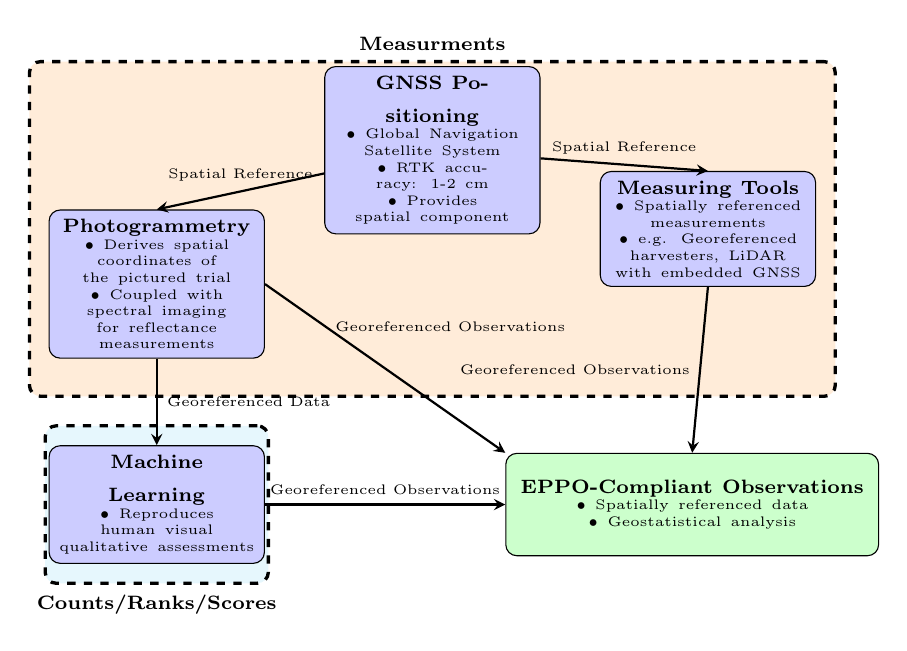
\begin{tikzpicture}[
            block/.style={rectangle, draw, fill=blue!20, text width=2.5cm, text centered, rounded corners, minimum height=1.3cm},
            arrow/.style={thick,->,>=stealth},
            groupbox/.style={rectangle, draw, rounded corners, very thick, dashed}
        ]
            
            % Background grouping rectangles
            % Light blue background for Visual assessments
            \node[groupbox, fill=cyan!10, text width=2.6cm, minimum height=2cm] (visual_group) at (-1,-2) {};
            \node[below] at (visual_group.south) {\scriptsize \textbf{Counts/Ranks/Scores}};
            
            % Light orange background for Continuous values
            \node[groupbox, fill=orange!15, text width=10cm, minimum height=4.25cm] (continuous_group) at (2.5,1.5) {};
            \node[above] at (continuous_group.north) {\scriptsize \textbf{Measurments}};
            
            % GNSS Block
            \node[block] (gnss) at (2.5,2.5) {
                \textbf{\scriptsize GNSS Positioning}\\
                \tiny
                $\bullet$ Global Navigation Satellite System\\
                $\bullet$ RTK accuracy: 1-2 cm\\
                $\bullet$ Provides spatial component\\
            };
            
            % Spectral Photogrammetry Block
            \node[block] (photogrammetry) at (-1,0.8) {
                \textbf{\scriptsize Photogrammetry}\\
                \tiny
                $\bullet$ Derives spatial coordinates of the pictured trial\\
                $\bullet$ Coupled with spectral imaging for reflectance measurements\\
            };
            
            % ML Inference Block
            \node[block] (ml) at (-1,-2) {
                \textbf{\scriptsize Machine Learning}\\
                \tiny
                $\bullet$ Reproduces human visual qualitative assessments\\
            };
            
            % Georeferenced Measuring Tools
            \node[block] (tools) at (6,1.5) {
                \textbf{\scriptsize Measuring Tools}\\
                \tiny
                $\bullet$ Spatially referenced measurements\\
                $\bullet$ e.g. Georeferenced harvesters, LiDAR with embedded GNSS\\
            };
            
            % Output Block
            \node[block, fill=green!20, text width=4.5cm] (output) at (5.8,-2) {
                \textbf{\scriptsize EPPO-Compliant Observations}\\
                \tiny
                $\bullet$ Spatially referenced data\\
                $\bullet$ Geostatistical analysis\\
            };

            % Arrows with proper syntax
            \draw[arrow] (gnss) -- (photogrammetry.north) node[midway,above] {\tiny Spatial Reference};
            \draw[arrow] (photogrammetry) -- (ml) node[midway,right] {\tiny Georeferenced Data};
            \draw[arrow] (ml.east) -- (output.west) node[midway,above] {\tiny Georeferenced Observations};
            \draw[arrow] (gnss) -- (tools.north) node[midway,above] {\tiny Spatial Reference};
            \draw[arrow] (tools.south) -- (output.north) node[midway,left] {\tiny Georeferenced Observations};
            \draw[arrow] (photogrammetry.east) -- (output.north west) node[near start,right] {\tiny Georeferenced Observations};
            % You can use [below], [above], [left], [right], [pos=0.5], [near start], [near end], [very near start], [very near end], [midway], [sloped], [bend left], [bend right], [out=angle], [in=angle], [loop], [shorten >=<length>], [shorten <=<length>], [looseness=<factor>], [distance=<length>], [swap], [auto], [anchor=<anchor>], [at end], [at start], [name path=<name>], [name intersections={of=<nameA> and <nameB>}], etc.
            % Example: \draw[->] (A) -- (B) node[midway, above] {Label};
        \end{tikzpicture}
    \end{center}

\end{frame}

% Slide 14: Georeferencing EPPO standard assessments
\begin{frame}
    \frametitle{Georeferencing EPPO Standard Assessments}
    
    \begin{table}[ht]
        \caption{\small EPPO's types of variables}
        \label{tab:data_types_slide}
        \centering
        \begin{tabular}{|l|c|c|c|}
        \hline
        \textbf{Type of Variable} & \textbf{Measurement} & \textbf{Ranking} & \textbf{Scoring} \\
        \hline
        \rowcolor{green!20} Continuous not limited & X & & \\
        \hline
        \rowcolor{green!20} Continuous limited & X & & \\
        \hline
        \rowcolor{yellow!20} Discrete & X & & \\
        \hline
        \rowcolor{red!20} Ordinal & & X & X \\
        \hline
        \rowcolor{red!20} Nominal & & & X \\
        \hline
        \rowcolor{red!20} Binary & & & X \\
        \hline
        \end{tabular}
        \end{table}
        
    \begin{flushleft}
        \hspace{1.5cm}{\tiny Summary from EPPO PP 1/152: Design and analysis of efficacy evaluation trials}
    \end{flushleft}

    \begin{block}{Current State of Georeferencing in Agricultural Trials:}
        \small Tool-based measurements (e.g., yield harvesters) can be easily georeferenced by integrating GNSS receivers on the tool. For visual assessments as counting, scoring or ranking, a method to transform georeferenced data to georeferenced observations is needed.
    \end{block}
\end{frame}

% Slide 15: ML Inference on Georeferenced Data
\begin{frame}
    \frametitle{Machine Learning Inference on Georeferenced Data}
    
    \begin{center}
        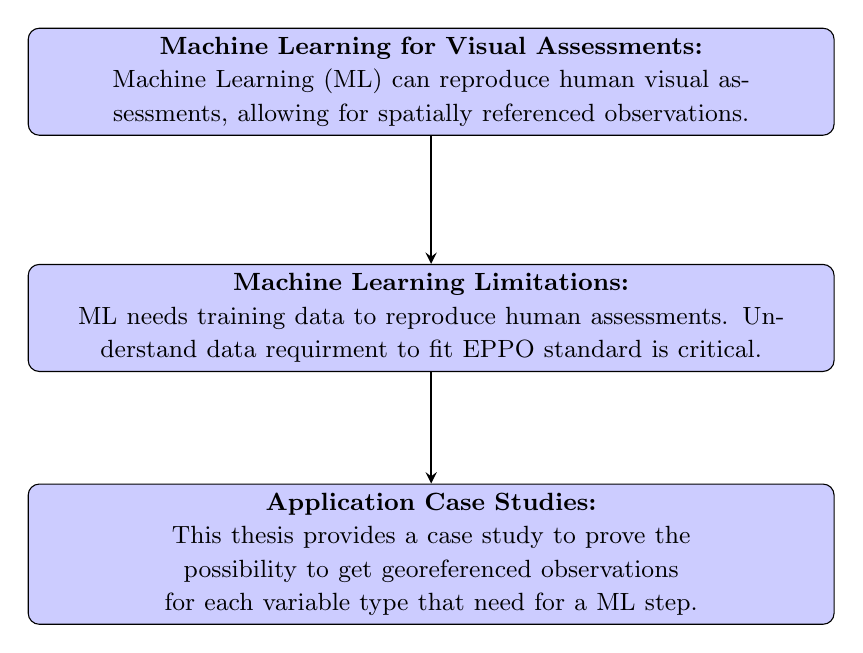
\begin{tikzpicture}[
            block/.style={rectangle, draw, fill=blue!20, text width=10cm, text centered, rounded corners, minimum height=1.3cm},
            arrow/.style={thick,->,>=stealth},
            groupbox/.style={rectangle, draw, rounded corners, very thick, dashed}
        ]
                        
            % First Block
            \node[block] (first) at (0,4) {
                \textbf{\small Machine Learning for Visual Assessments:}\\
            \small Machine Learning (ML) can reproduce human visual assessments, allowing for spatially referenced observations.        
            };
            % Second Block
            \node[block] (second) at (0,1) {
                \textbf{\small Machine Learning Limitations:}\\
            \small ML needs training data to reproduce human assessments. Understand data requirment to fit EPPO standard is critical.        
            };
            % Third Block
            \node[block] (third) at (0,-2) {
                \textbf{\small Application Case Studies:}\\
            \small This thesis provides a case study to prove the possibility to get georeferenced observations for each variable type that need for a ML step.         
            };

            % Arrows with proper syntax
            \draw[arrow] (first.south) -- (second.north);
            \draw[arrow] (second.south) -- (third.north);

        \end{tikzpicture}
    \end{center}
\end{frame}

% Slide 15: EPPO ML integration
\begin{frame}
    \frametitle{EPPO ML integration}
    
    \begin{block}{EPPO PP 1/333(1): Digital Technologies in PPP Trials}
        \small
        ML integrated assessments must meet the same quality standards as manual assessments and require validation through comparison with manual assessments (golden sample).
    \end{block}
    
    \begin{exampleblock}{\small Validation Benchmarks\footnote{\tiny Based on EPPO PP 1/333(1): Use of digital technologies in efficacy and selectivity trials}}
        \scriptsize
        \begin{itemize}
            \item \textbf{\large Continuous/Discrete}\large : $R^2 > 0.85$ (1:1 relationship)
            \item \textbf{\large Ordinal/Nominal}\large : Cohen's $\kappa > 0.7$
            \item \textbf{\large Binary}\large : Accuracy $> 0.85$
        \end{itemize}
    \end{exampleblock}
\end{frame}

% Slide 16: Georeferencing EPPO Standard Assessments: Case Studies
\begin{frame}
    \frametitle{Georeferencing Gap in EPPO Standard Assessments}
    \begin{table}[ht]
        \centering
        \begin{tabular}{|c|l|c|c|c|}
        \hline
        & \textbf{Type of Variable} & \textbf{Measurement} & \textbf{Ranking} & \textbf{Scoring} \\
        \hline
        \rowcolor{green!20} & Continuous not limited & X & & \\
        \hline
        \rowcolor{green!20} & Continuous limited & X & & \\
        \hline
        \rowcolor{yellow!20} $\rightarrow$ & Discrete & X & & \\
        \hline
        \rowcolor{red!20} $\rightarrow$ & Ordinal & & X & X \\
        \hline
        \rowcolor{red!20} $\rightarrow$ & Nominal & & & X \\
        \hline
        \rowcolor{red!20} $\rightarrow$ & Binary & & & X \\
        \hline
        \end{tabular}
    \end{table}
    \begin{block}{Case Studies:}
        \small This thesis aim to prove the reliability of georeferencing every EPPO standard assessmentEach case study addresses a specific variable type as defined in the EPPO standards
        \begin{itemize}
            \item \textbf{Discrete (Counts)} : Plant counting
            \item \textbf{Ordinal} : Phytotoxicity scoring
            \item \textbf{Nominal} and \textbf{Binary} : Disease detection 
        \end{itemize}
    \end{block}
\end{frame}

% Slide 17: Georeferencing Counts (Discrete Variable) 
\begin{frame}
    \frametitle{Georeferencing Counts (Discrete Variable)}
    \begin{table}[ht]
        \centering
        \begin{tabular}{|c|l|c|c|c|}
        \hline
        & \textbf{Type of Variable} & \textbf{Measurement} & \textbf{Ranking} & \textbf{Scoring} \\
        \hline
        \rowcolor{green!20} & Continuous not limited & X & & \\
        \hline
        \rowcolor{green!20} & Continuous limited & X & & \\
        \hline
        \rowcolor{yellow!20} $\rightarrow$ & Discrete & X & & \\
        \hline
        \rowcolor{red!20} & Ordinal & & X & X \\
        \hline
        \rowcolor{red!20} & Nominal & & & X \\
        \hline
        \rowcolor{red!20} & Binary & & & X \\
        \hline
        \end{tabular}
    \end{table}
    \begin{block}{Georeferencing Counts:}
        \small
        \begin{itemize}
            \item \textbf{Counts} are discrete variables required for measuring density of individuals (e.g. plant density in PP1/46 (3) - Wireworms).
            \item the \textbf{Case Study}: Counting plants from georeferenced photogrammetric orthomosaics by ML Object Detection. 
            \item this study is discussed in the scientific article \textbf{\scriptsize Bumbaca, S.; Borgogno-Mondino, E.C. On the Minimum Dataset Requirements for Fine-Tunining an Object Detector for Arable Crop Plant Counting: A Case Study on Maize Seedlings. Remote Sens. 2025, 17, 2190. DOI: 10.3390/rs1713219061}
        \end{itemize}
    \end{block}
\end{frame}

% PLANT COUNTING CASE STUDY

% Slide 18: Plant Counting Introduction - The Problem
\begin{frame}
    \frametitle{Plant Counting: The Core Challenge}
    
    \begin{block}{The Critical Need after EPPO Assessments:}
        \begin{itemize}
            \item Plant counting is \textbf{fundamental} in precision agriculture and plant breeding
            \item Traditional manual counting is \textbf{time-consuming} and \textbf{variable}
            \item Computer vision offers automation and standardization but requires \textbf{dataset size and quality} characterization to prove the reliability for this task.
        \end{itemize}
    \end{block}
    
    \begin{exampleblock}{EPPO Benchmark Standards:}
        Coefficient of determination ($R^2$) $\geq$ 0.85 w.r.t. manual counting
    \end{exampleblock}
    
    \begin{alertblock}{Research Gap:}
        \textit{What are the minimum dataset requirements to achieve these benchmarks across different inference datasets?}
    \end{alertblock}
\end{frame}

% Slide 19: Plant Counting - Case Study Selection
\begin{frame}
    \frametitle{Case Study: Maize Seedling Counting}
    
    \begin{block}{Why Maize Seedlings?}
        \small
        \begin{itemize}
            \item \textbf{Data availability}: Most represented plant in scientific \fcite{\citeDavid} \fcite{\citeLiu} and public datasets \fcite{\citeMaizeSeeding} \fcite{\citeMaizeSeedling}
            \item \textbf{Economic importance}: Most important crop worldwide by production \fcite{\citeFAO}
            \item \textbf{Optimal detection conditions}: Low overlapping and fixed spacing at V3-V5 stage
        \end{itemize}
    \end{block}
    
    \begin{columns}
        \begin{column}{0.5\textwidth}
            \begin{exampleblock}{Growth Stage Selection:}
                \small
                \textbf{V3-V5 (BBCH 13-15)} \fcite{\citeMeier}
                \begin{itemize}
                    \item 3rd-5th leaf unfolded
                    \item Fixed intra-row and inter-row spacing
                    \item Minimal plant overlapping
                \end{itemize}
            \end{exampleblock}
        \end{column}
        
        \begin{column}{0.5\textwidth}
            \begin{alertblock}{Broader Applications:}
                \small
                Similar detection challenges in other row crops:
                \begin{itemize}
                    \item \textbf{Sunflower} (Helianthus annuus L.)
                    \item \textbf{Sugar beet} (Beta vulgaris L.)
                    \item Other crops with inter-row spacing
                \end{itemize}
            \end{alertblock}
        \end{column}
    \end{columns}
\end{frame}

% Slide 20: Plant Counting - Object Detection Evolution
\begin{frame}
    \frametitle{Object Detection Approaches: From Handcrafted to Deep Learning}
    
    \begin{block}{Handcrafted Methods (HC):}
        \small
        \begin{itemize}
            \item \textbf{Traditional approach}: Still used in agricultural applications \fcite{\citeDavid} \fcite{\citeGarcia}
            \item \textbf{Color thresholding} in HSV space + morphological operations
            \item \textbf{Trade-off}: High precision on subset vs. limited generalizability
        \end{itemize}
    \end{block}
    
    \begin{columns}
        \begin{column}{0.5\textwidth}
            \begin{exampleblock}{CNN-based Models:}
                \small
                \textbf{Convolutional Neural Networks} \fcite{\citeLeCun}
                \begin{itemize}
                    \item \textbf{YOLO family}: YOLOv5, YOLOv8
                    \item \textbf{Faster R-CNN} \fcite{\citeFasterRCNN}
                    \item Grid-like image processing
                    \item Efficient for small images
                \end{itemize}
            \end{exampleblock}
        \end{column}
        
        \begin{column}{0.5\textwidth}
            \begin{exampleblock}{Transformer-based:}
                \small
                \textbf{Attention mechanisms} \fcite{\citeVaswani}
                \begin{itemize}
                    \item \textbf{DETR} \fcite{\citeCarion}
                    \item \textbf{RT-DETR}: Real-time performance
                    \item Sequence of patches processing
                    \item Superior with scarce data \fcite{\citeRekavandi}
                \end{itemize}
            \end{exampleblock}
        \end{column}
    \end{columns}
    
    \begin{alertblock}{Key Insight:}
        \small Transformer-based models outperform CNN-based on common benchmarks \fcite{\citeZong} and show better fine-tuning performance with limited data
    \end{alertblock}
\end{frame}

% Slide 21: Plant Counting - YOLO vs RT-DETR Architecture
\begin{frame}
    \frametitle{Representative Architectures: YOLO vs RT-DETR}
    
    \begin{columns}
        \begin{column}{0.5\textwidth}
            \begin{block}{YOLO Family (Pure CNN):}
                \small
                \textbf{Why chosen as representatives:}
                \begin{itemize}
                    \item \textbf{Large adoption} in agriculture \fcite{\citeBadgujar}
                    \item \textbf{Good precision} and low dataset requirements vs. other CNNs \fcite{\citeTan} \fcite{\citeZhang}
                    \item \textbf{Speed-accuracy} optimizations
                \end{itemize}
                
                \textbf{Variants tested:}
                \begin{itemize}
                    \item \textbf{YOLOv5}: CSPDarknet53 backbone
                    \item \textbf{YOLOv8}: Improved architecture with decoupled head
                \end{itemize}
            \end{block}
        \end{column}
        
        \begin{column}{0.5\textwidth}
            \begin{exampleblock}{RT-DETR (Transformer-mixed):}
                \small
                \textbf{Why chosen:}
                \begin{itemize}
                    \item \textbf{Outperforms} YOLOv5 and YOLOv8 \fcite{\citeZhao}
                    \item \textbf{Real-time} transformer detector
                    \item \textbf{Hybrid approach}: CNN backbone + transformer decoder
                \end{itemize}
                
                \textbf{Architecture advantages:}
                \begin{itemize}
                    \item Enhanced feature extraction
                    \item Better handling of spatial relationships
                    \item Improved performance with limited data
                \end{itemize}
            \end{exampleblock}
        \end{column}
    \end{columns}
    
    \begin{block}{Emerging Paradigms:}
        \small
        \textbf{Zero-shot} \fcite{\citeBansal} and \textbf{few-shot} \fcite{\citeHuang} detection aim to reduce annotation burden through semantic relationships and meta-learning
    \end{block}
\end{frame}

% Slide 22: Plant Counting - Dataset Requirements Challenge
\begin{frame}
    \frametitle{The Dataset Requirements Challenge in Agriculture}
    
    \begin{alertblock}{Critical Research Gap:}
        \small
        Few studies focus on minimum dataset requirements for robust plant detectors \fcite{\citeDavid} \fcite{\citeAndvaag}, despite extensive work on agricultural object detection \fcite{\citeBarreto} \fcite{\citeJiang} \fcite{\citeLiu}
    \end{alertblock}
    
    \begin{block}{Known Performance Factors:}
        \small
        \begin{itemize}
            \item \textbf{Dataset size}: Performance directly related to training data amount \fcite{\citeSun}
            \item \textbf{Data quality}: Annotation accuracy critically affects model performance \fcite{\citeAlhazmi}
            \item \textbf{Model architecture}: Different models require different dataset sizes for same performance \fcite{\citeNguyen} \fcite{\citeBrigato}
        \end{itemize}
    \end{block}
    
    \begin{columns}
        \begin{column}{0.5\textwidth}
            \begin{exampleblock}{Domain-Specific Factors:}
                \small
                \begin{itemize}
                    \item \textbf{Backbone importance} \fcite{\citeDu}
                    \item \textbf{Domain-specific pre-training} benefits \fcite{\citeRoggiolani}
                    \item \textbf{Data augmentation} strategies \fcite{\citeShorten}
                \end{itemize}
            \end{exampleblock}
        \end{column}
        
        \begin{column}{0.5\textwidth}
            \begin{alertblock}{Most Critical Factor:}
                \small
                \textbf{Dataset source} \fcite{\citeSun}: In-domain vs. out-of-distribution dramatically affects accuracy and dataset size requirements \fcite{\citeDavid} \fcite{\citeAndvaag}
            \end{alertblock}
        \end{column}
    \end{columns}
\end{frame}

% Slide 23: Plant Counting Introduction - Object Detection Approaches
\begin{frame}
    \frametitle{Object Detection Paradigms for Plant Counting}
    
    \begin{columns}
        \begin{column}{0.5\textwidth}
            \begin{block}{Many-Shot Models:}
                \small
                \begin{itemize}
                    \item \textbf{CNN-based}: YOLOv5, YOLOv8
                    \item \textbf{Transformer-mixed}: RT-DETR, YOLO11
                    \item Require extensive labeled datasets
                    \item State-of-the-art performance
                \end{itemize}
            \end{block}
            
            \begin{block}{Few-Shot Models:}
                \small
                \begin{itemize}
                    \item \textbf{CD-ViTO}: Cross-domain adaptation
                    \item Meta-learning approaches
                    \item 1-50 training examples
                    \item Promising but unvalidated for agriculture
                \end{itemize}
            \end{block}
        \end{column}
        
        \begin{column}{0.5\textwidth}
            \begin{block}{Zero-Shot Models:}
                \small
                \begin{itemize}
                    \item \textbf{OWLv2}: Open-vocabulary detection
                    \item Vision-language foundation models
                    \item Text prompt-based detection
                    \item No training data required
                \end{itemize}
            \end{block}
            
            \begin{block}{Handcrafted Methods:}
                \small
                \begin{itemize}
                    \item \textbf{Color thresholding} + agronomic knowledge
                    \item High precision in constrained scenarios
                    \item Still used as baseline/annotation tool
                    \item Limited generalizability
                \end{itemize}
            \end{block}
        \end{column}
    \end{columns}
\end{frame}

% Slide 24: Plant Counting Introduction - Study Objectives
\begin{frame}
    \frametitle{Study Objectives and Research Questions}
    
    \begin{exampleblock}{Primary Objective:}
        Determine minimum dataset size and quality required to achieve EPPO benchmarks (R² $\geq$ 0.85) for maize seedling detection across different object detection paradigms.
    \end{exampleblock}
    
    \begin{block}{Specific Research Questions:}
        \begin{enumerate}
            \item What is the impact of \textbf{dataset source} (in-domain vs. out-of-distribution)?
            \item How do \textbf{model architectures} affect dataset requirements?
            \item What is the minimum acceptable \textbf{annotation quality}?
            \item Can \textbf{few-shot/zero-shot} approaches meet agricultural benchmarks?
            \item What role do \textbf{handcrafted methods} play in the DL era?
        \end{enumerate}
    \end{block}
    
    \begin{alertblock}{Case Study Focus:}
        \textbf{Maize seedlings} (Zea mays L.) at V3-V5 growth stage from georeferenced orthomosaics
    \end{alertblock}
\end{frame}

% Slide 25: Materials and Methods - Dataset Overview
\begin{frame}
    \frametitle{Dataset Collection and Preparation}
    
    \begin{columns}
        \begin{column}{0.6\textwidth}
            \begin{block}{Dataset Sources:}
                \small
                \textbf{Out-of-Distribution (OOD):}
                \begin{itemize}
                    \item Scientific literature: 778 tiles
                    \item Internet repositories: 390 tiles
                    \item Pre-annotated datasets
                \end{itemize}
                
                \textbf{In-Domain (ID):}
                \begin{itemize}
                    \item 3 study sites: 450 training + 60 test tiles
                    \item Phantom 4 Pro v2.0 @ 10m AGL
                    \item Bundle adjustment error: 38mm (GNSS VRS-NRTK)
                \end{itemize}
            \end{block}
        \end{column}
        
        \begin{column}{0.4\textwidth}
            \begin{block}{Technical Specs:}
                \small
                \begin{itemize}
                    \item \textbf{Resolution}: 5 mm/pixel
                    \item \textbf{Tile size}: 224×224 pixels
                    \item \textbf{Coverage}: 1.12×1.12 meters
                    \item \textbf{Content}: ~2 maize rows per tile
                    \item \textbf{Annotation}: Squared bounding boxes centered on stems
                \end{itemize}
            \end{block}
            
            \begin{alertblock}{\small Key Insight:}
                \small Tile size optimized for row pattern identification and model compatibility
            \end{alertblock}
        \end{column}
    \end{columns}
\end{frame}

% Slide 26: Materials and Methods - Handcrafted Algorithm
\begin{frame}
    \frametitle{Handcrafted Object Detector: Two-Stage Pipeline}
    
    \begin{columns}
        \begin{column}{0.5\textwidth}
            \begin{block}{Stage 1 - HC1 (Detection):}
                \small
                \begin{enumerate}
                    \item \textbf{Color thresholding} in HSV space
                    \item \textbf{Connected components} analysis
                    \item \textbf{Size filtering} based on leaf area
                    \item Outputs: Potential plant regions
                \end{enumerate}
                
                \textit{Result: High recall, many false positives}
            \end{block}
            
            \begin{block}{Stage 2 - HC2 (Verification):}
                \small
                \begin{enumerate}
                    \item \textbf{RANSAC} line fitting for row detection
                    \item \textbf{Row spacing} validation
                    \item \textbf{Plant count} verification per row
                    \item \textbf{Agronomic knowledge} application
                \end{enumerate}
                
                \textit{Result: High precision, limited coverage}
            \end{block}
        \end{column}
        
        \begin{column}{0.5\textwidth}
            \begin{exampleblock}{Algorithm Performance:}
                \small
                \begin{table}[h]
                    \scriptsize
                    \begin{tabular}{lccc}
                        \textbf{Dataset} & \textbf{R²} & \textbf{Coverage} \\
                        \hline
                        ID\_1 & 0.95 & 7.8\% \\
                        ID\_2 & 0.93 & 4.2\% \\
                        ID\_3 & 0.87 & 1.8\% \\
                    \end{tabular}
                \end{table}
            \end{exampleblock}
            
            \begin{alertblock}{\small Trade-off:}
                Excellent accuracy on subset of data vs. limited generalizability
            \end{alertblock}
        \end{column}
    \end{columns}
\end{frame}

% Slide 27: Materials and Methods - Deep Learning Models
\begin{frame}
    \frametitle{Deep Learning Model Configuration}
    
    \begin{block}{Many-Shot Models (Ultralytics Implementation):}
        \small
        \begin{columns}
            \begin{column}{0.5\textwidth}
                \textbf{CNN-based:}
                \begin{itemize}
                    \item YOLOv5 (n, s, m, l, x)
                    \item YOLOv8 (n, s, m, l, x)
                \end{itemize}
                
                \textbf{Transformer-mixed:}
                \begin{itemize}
                    \item YOLO11 (n, s, m, l, x)
                    \item RT-DETR (l, x)
                \end{itemize}
            \end{column}
            
            \begin{column}{0.5\textwidth}
                \textbf{Training Settings:}
                \begin{itemize}
                    \item Batch size: 16
                    \item Max epochs: 200
                    \item Early stopping: 15 epochs
                    \item Mixed precision training
                    \item Default Ultralytics augmentation
                \end{itemize}
            \end{column}
        \end{columns}
    \end{block}
    
    \begin{columns}
        \begin{column}{0.5\textwidth}
            \begin{block}{Few-Shot: CD-ViTO}
                \small
                \begin{itemize}
                    \item ViT-S/B/L backbones (22M/86M/307M params)
                    \item 1, 5, 10, 30, 50 shots tested
                    \item Cross-domain adaptation
                \end{itemize}
            \end{block}
        \end{column}
        
        \begin{column}{0.5\textwidth}
            \begin{block}{Zero-Shot: OWLv2}
                \small
                \begin{itemize}
                    \item ViT-B/16, ViT-L/14 encoders
                    \item Base, fine-tuned, ensemble variants
                    \item 11 different text prompts tested
                \end{itemize}
            \end{block}
        \end{column}
    \end{columns}
\end{frame}

% Slide 28: Materials and Methods - Experimental Design
\begin{frame}
    \frametitle{Experimental Design and Evaluation Metrics}
    
    \begin{block}{Dataset Size Investigation:}
        \small
        \begin{itemize}
            \item \textbf{Many-shot}: 10-150 images in steps of 10
            \item \textbf{Few-shot}: 1, 5, 10, 30, 50 shots
            \item \textbf{Zero-shot}: No training data required
        \end{itemize}
    \end{block}
    
    \begin{block}{Dataset Quality Investigation:}
        \small
        Annotation quality reduced from 100\% to 10\% in 10\% steps for successful models
    \end{block}
    
    \begin{columns}
        \begin{column}{0.5\textwidth}
            \begin{exampleblock}{Evaluation Metrics:}
                \small
                \textbf{Counting Performance:}
                \begin{itemize}
                    \item $R^2$ (coefficient of determination)
                    \item $RMSE$ (root mean square error)
                    \item $MAPE$ (mean absolute percentage error)
                \end{itemize}
                
                \textbf{Detection Performance:}
                \begin{itemize}
                    \item $mAP$ @ IoU 0.5
                \end{itemize}
            \end{exampleblock}
        \end{column}
        
        \begin{column}{0.5\textwidth}
            \begin{exampleblock}{Performance Modeling:}
                \small
                Empirical functions tested:
                \begin{itemize}
                    \item $f(x) = a \ln(x) + b$
                    \item $f(x) = a \arctan(bx) + c$
                    \item $f(x) = a x^{1/b} + c$
                \end{itemize}
                
                Best fit selected by $R^2_{fit}$ (GoF)
            \end{exampleblock}
        \end{column}
    \end{columns}
\end{frame}

% Slide 29: Materials and Methods - Testing Protocol
\begin{frame}
    \frametitle{Testing Protocol and Infrastructure}
    
    \begin{block}{Hardware Configuration:}
        \small
        \begin{itemize}
            \item \textbf{CPU}: Intel Xeon E5-2670 v3 @ 2.30GHz
            \item \textbf{RAM}: 64.0 GB
            \item \textbf{GPU}: NVIDIA RTX A5000 (24GB VRAM)
            \item \textbf{Implementation}: Ultralytics, HuggingFace Transformers
        \end{itemize}
    \end{block}
    
    \begin{columns}
        \begin{column}{0.6\textwidth}
            \begin{block}{SAHI Testing Method:}
                \small
                \begin{enumerate}
                    \item \textbf{Slice}: Test images into overlapping patches
                    \item \textbf{Detect}: Run model on each patch
                    \item \textbf{Merge}: Combine predictions with NMS
                    \item \textbf{Threshold}: Apply confidence score filtering
                \end{enumerate}
                
                \textit{Rationale: Handles object occlusion at tile boundaries}
            \end{block}
        \end{column}
        
        \begin{column}{0.4\textwidth}
            \begin{exampleblock}{Confidence Thresholds:}
                \scriptsize
                0, 0.05, 0.1, 0.15, 0.2, 0.25, 0.29, 0.4, 0.5, 0.6, 0.7, 0.8, 0.9, 0.95, 0.99
                
                \vspace{0.3cm}
                \textbf{Best R² selected} across all thresholds for each model
            \end{exampleblock}
        \end{column}
    \end{columns}
    
    \begin{alertblock}{Key Principle:}
        \small All models tested on same ID test dataset (20 tiles × 3 locations = 60 tiles total)
    \end{alertblock}
\end{frame}

% Slide 30: Results - OOD vs ID Performance
\begin{frame}
    \frametitle{Critical Impact of Dataset Source}
    
    \begin{alertblock}{Major Finding:}
        \large \textbf{NO} out-of-distribution model achieved benchmark performance ($R^2 \geq$ 0.85)
    \end{alertblock}
    
    \begin{columns}
        \begin{column}{0.5\textwidth}
            \begin{block}{OOD Results:}
                \small
                \begin{itemize}
                    \item \textbf{Best R²}: < 0.5 (all models)
                    \item \textbf{Best MAPE}: ~20% (still insufficient)
                    \item \textbf{GoF values}: < 0.2 (poor predictability)
                    \item \textbf{Dataset size}: Up to 1,168 images tested
                \end{itemize}
            \end{block}
            
            \begin{alertblock}{Domain Gap Challenge:}
                \small
                \begin{itemize}
                    \item Environmental conditions
                    \item Lighting variations
                    \item Camera parameters
                    \item Plant growth stages
                \end{itemize}
            \end{alertblock}
        \end{column}
        
        \begin{column}{0.5\textwidth}
            \begin{exampleblock}{ID Success Stories:}
                \small
                \textbf{Models achieving $R^2 \geq$ 0.85:}
                \begin{itemize}
                    \item YOLOv5n: 130 samples
                    \item YOLOv5s: 130 samples  
                    \item YOLOv8n: 110 samples
                    \item RT-DETR L: 60 samples
                    \item RT-DETR X: 100 samples
                \end{itemize}
                
                \textbf{GoF values}: > 0.3 (high predictability)
            \end{exampleblock}
        \end{column}
    \end{columns}
    
    \begin{block}{Practical Implication:}
        \small In-domain data collection is \textbf{non-negotiable} for agricultural applications
    \end{block}
\end{frame}

% Slide 31: Results - Architecture Comparison
\begin{frame}
    \frametitle{Architecture-Specific Dataset Requirements}
    
    \begin{columns}
        \begin{column}{0.6\textwidth}
            \begin{block}{CNN-based Models (YOLO family):}
                \small
                \begin{itemize}
                    \item \textbf{YOLOv5n}: 130 samples (1.9M params)
                    \item \textbf{YOLOv5s}: 130 samples (7.2M params)
                    \item \textbf{YOLOv8n}: 110 samples (3.2M params)
                \end{itemize}
                
                \textit{Pattern: Larger models → more samples needed}
            \end{block}
            
            \begin{exampleblock}{Transformer-mixed Models:}
                \small
                \begin{itemize}
                    \item \textbf{RT-DETR L}: 60 samples (60M params)
                    \item \textbf{RT-DETR X}: 100 samples (80M params)
                \end{itemize}
                
                \textit{RT-DETR L most efficient}
            \end{exampleblock}
        \end{column}
        
        \begin{column}{0.4\textwidth}
            \begin{block}{Key Insights:}
                \small
                \begin{itemize}
                    \item \textbf{Transformers more sample-efficient} than CNNs
                    \item \textbf{Long-range dependencies} better captured
                    \item \textbf{Trade-off}: Higher computational cost
                \end{itemize}
            \end{block}
            
            \begin{alertblock}{Practical Decision:}
                \scriptsize
                \textbf{CNN approach}: 
                Collect ~130 samples + lower compute
                
                \textbf{Transformer approach}: 
                Collect ~60 samples + higher compute
            \end{alertblock}
        \end{column}
    \end{columns}
    
    \begin{block}{Performance Predictability:}
        \small Logarithmic relationship between dataset size and performance enables resource planning (GoF > 0.3 for successful models)
    \end{block}
\end{frame}

% Slide 32: Results - Quality vs Quantity Trade-offs
\begin{frame}
    \frametitle{Dataset Quality Requirements}
    
    \begin{block}{Quality Tolerance Analysis:}
        Models achieving benchmark with reduced annotation quality:
    \end{block}
    
    \begin{columns}
        \begin{column}{0.5\textwidth}
            \begin{exampleblock}{Successful Quality Reductions:}
                \small
                \begin{itemize}
                    \item \textbf{YOLOv5n}: 85\% quality (130 samples)
                    \item \textbf{YOLOv5s}: 90\% quality (130 samples)
                    \item \textbf{YOLOv8n}: 85\% quality (110 samples)
                    \item \textbf{RT-DETR X}: 65\% quality (100 samples)
                \end{itemize}
            \end{exampleblock}
            
            \begin{alertblock}{RT-DETR L Sensitivity:}
                \small Failed to maintain benchmark with ANY quality reduction (60 samples baseline)
            \end{alertblock}
        \end{column}
        
        \begin{column}{0.5\textwidth}
            \begin{block}{Quality-Quantity Relationship:}
                \small
                \textbf{Key Finding}: Smaller datasets are more sensitive to annotation errors
                
                \textbf{RT-DETR L}: Minimal dataset (60 samples) → Each annotation critical
                
                \textbf{RT-DETR X}: Larger dataset (100 samples) → Error redundancy tolerance
            \end{block}
            
            \begin{exampleblock}{Practical Strategy:}
                \scriptsize
                \textbf{Option 1}: Perfect annotations + minimal dataset
                
                \textbf{Option 2}: Good quality annotations + larger dataset
                
                \textbf{Option 3}: Semi-automated annotation workflows
            \end{exampleblock}
        \end{column}
    \end{columns}
\end{frame}

% Slide 33: Results - Few-shot and Zero-shot Limitations
\begin{frame}
    \frametitle{Few-Shot and Zero-Shot: Current Limitations}
    
    \begin{alertblock}{Major Finding:}
        \large Neither few-shot nor zero-shot approaches achieved benchmark performance
    \end{alertblock}
    
    \begin{columns}
        \begin{column}{0.5\textwidth}
            \begin{block}{Few-Shot Results (CD-ViTO):}
                \small
                \textbf{Best Performance} (ViT-B, 50 shots):
                \begin{itemize}
                    \item \textbf{RMSE}: 3.9 (vs. benchmark 0.39)
                    \item \textbf{MAPE}: ~25%
                    \item \textbf{mAP}: ~0.5
                    \item \textbf{Error rate}: ~1 plant in 4 miscounted
                \end{itemize}
                
                \textit{Pattern: Performance plateaus after 30 shots}
            \end{block}
        \end{column}
        
        \begin{column}{0.5\textwidth}
            \begin{block}{Zero-Shot Results (OWLv2):}
                \small
                \begin{itemize}
                    \item \textbf{R²}: Always < 0 (worse than mean prediction)
                    \item \textbf{RMSE}: 5-25 (extremely high)
                    \item \textbf{MAPE}: 40-140\%
                    \item \textbf{Prompt sensitivity}: High variability across 11 prompts
                \end{itemize}
            \end{block}
        \end{column}
    \end{columns}
    
    \begin{block}{Why the Poor Performance?}
        \small
        \begin{itemize}
            \item \textbf{Domain specificity}: Aerial agricultural imagery differs from general object detection
            \item \textbf{Subtle features}: Intra-class variability in seedling appearance
            \item \textbf{Pre-training gap}: Models not optimized for agricultural tasks
            \item \textbf{Fine-grained detection}: Requires precise localization and counting
        \end{itemize}
    \end{block}
\end{frame}

% Slide 34: Discussion - Hybrid Approaches
\begin{frame}
    \frametitle{The Value of Hybrid Approaches}
    
    \begin{columns}
        \begin{column}{0.5\textwidth}
            \begin{block}{Handcrafted Method Performance:}
                \small
                \textbf{Strengths}:
                \begin{itemize}
                    \item R² = 0.87-0.95 (excellent accuracy)
                    \item RMSE = 0.11-0.18 (below benchmark)
                    \item Domain knowledge integration
                    \item High precision when applicable
                \end{itemize}
                
                \textbf{Limitations}:
                \begin{itemize}
                    \item Coverage: 1.8-7.8\% of tiles only
                    \item Color-thresholding bias
                    \item Limited generalizability
                \end{itemize}
            \end{block}
        \end{column}
        
        \begin{column}{0.5\textwidth}
            \begin{exampleblock}{Hybrid Strategy Potential:}
                \small
                \textbf{1. Bootstrap Training}:
                \begin{itemize}
                    \item HC method generates high-quality annotations
                    \item Deep learning models trained on HC output
                    \item Overcomes manual annotation bottleneck
                \end{itemize}
                
                \textbf{2. Quality Filtering}:
                \begin{itemize}
                    \item OOD/few-shot/zero-shot occasional good predictions
                    \item HC2 validates agronomic patterns
                    \item Reduces color-thresholding bias
                \end{itemize}
            \end{exampleblock}
        \end{column}
    \end{columns}
    
    \begin{alertblock}{Future Work Direction:}
        \small Develop automated methods to identify and leverage high-quality annotations from sub-benchmark models using agronomic validation
    \end{alertblock}
\end{frame}

% Slide 35: Discussion - Practical Implications
\begin{frame}
    \frametitle{Practical Implementation Guidelines}
    
    \begin{block}{Resource Optimization Strategy:}
        \small
        \textbf{Step 1}: Focus on minimum viable dataset size (60-130 images)
        \textbf{Step 2}: Logarithmic relationship → diminishing returns beyond minimum
        \textbf{Step 3}: Quality vs. quantity trade-off consideration
    \end{block}
    
    \begin{columns}
        \begin{column}{0.5\textwidth}
            \begin{exampleblock}{Implementation Pathways:}
                \scriptsize
                \textbf{High-Resource Scenario}:
                \begin{itemize}
                    \item RT-DETR L + 60 perfect annotations
                    \item Higher computational investment
                    \item Fastest deployment
                \end{itemize}
                
                \textbf{Medium-Resource Scenario}:
                \begin{itemize}
                    \item YOLOv8n + 110 good annotations
                    \item Balanced compute/annotation effort
                    \item Robust performance
                \end{itemize}
                
                \textbf{Low-Resource Scenario}:
                \begin{itemize}
                    \item YOLOv5n + 130 annotations (85\% quality)
                    \item Semi-automated annotation
                    \item Cost-effective solution
                \end{itemize}
            \end{exampleblock}
        \end{column}
        
        \begin{column}{0.5\textwidth}
            \begin{block}{Critical Success Factors}
                \small
                \begin{enumerate}
                    \item \textbf{In-domain data}: Non-negotiable requirement
                    \item \textbf{Architecture choice}: Based on resource constraints
                    \item \textbf{Quality assessment}: Monitor annotation accuracy
                    \item \textbf{Validation protocol}: SAHI testing recommended
                \end{enumerate}
            \end{block}
            
            \begin{alertblock}{Industry Adoption}
                \scriptsize Current few-shot/zero-shot methods not ready for production agricultural applications
            \end{alertblock}
        \end{column}
    \end{columns}
\end{frame}

% Slide 36: Conclusions
\begin{frame}
    \frametitle{Conclusions: Evidence-Based Guidelines for Agricultural Object Detection}
    
    \begin{exampleblock}{Core Findings}
        \begin{itemize}
            \item \textbf{In-domain training data is mandatory} - OOD approaches fail to achieve benchmarks
            \item \textbf{Architecture matters}: Transformer-mixed models (RT-DETR) require 50\% fewer samples than CNN-based models
            \item \textbf{Quality tolerance exists}: Models maintain performance with 65-90\% annotation quality
            \item \textbf{Current limitations}: Few-shot and zero-shot methods cannot meet precision agriculture requirements
        \end{itemize}
    \end{exampleblock}
    
    \begin{block}{Practical Contributions}
        \begin{itemize}
            \item \textbf{Minimum dataset requirements established}: 60-130 samples depending on architecture
            \item \textbf{Predictable performance scaling}: Logarithmic relationship enables resource planning
            \item \textbf{Hybrid approach potential}: Handcrafted methods valuable for annotation bootstrapping
            \item \textbf{Quality-quantity trade-offs quantified}: Strategic annotation workflow optimization
        \end{itemize}
    \end{block}
    
    \begin{alertblock}{Impact and Future Work}
        These findings provide \textbf{evidence-based guidance} for implementing maize seedling detection systems and suggest \textbf{domain-specific pre-training} as a promising direction for further reducing dataset requirements.
    \end{alertblock}
\end{frame}

\end{document}
